\section{Evaluation}
\label{sec:evaluation}

In this section we present the results obtained for both CPU and GPU
implementations and analyze the speedup obtained when applying the
optimizations described in Section~\ref{sec:op_strategies}.

Our test system is a quad-core Intel Core i7-920 running at 2.67 GHz with
Hyper-threading enabled. For compilation we used \textit{gcc 4.6} with flags
``-O3 -march=native -funroll-loops -fargument-noalias -fopenmp''. The GPU cards
used were GeForce GTX 480 from Nvidia (Fermi architecture) having 1.5 GB of
total memory and 15 multiprocessors each with 32 lanes operating at a clock
speed of 1.4 GHz. For programming the GPUs, we started from the CPU code base
and implemented the algorithms and optimizations with the established CUDA
framework, making use of specific Nvidia features. An important observation to
make is that the device supports CUDA Capability 2.0 which, among other
features, includes the possibility for the same on-chip memory to be used for
both L1 cache and shared memory. It can be configured as either 48 KB of shared
memory and 16 KB of L1 cache or as 16 KB of shared memory and 48 KB of L1 cache.
We used the second option for the \textit{evaluation} algorithm in order to
cache the accesses to local and global memory and also temporary register
spills. For compilation, we used \textit{Cuda Toolkit 4.1} with flags
``-arch=sm\_20''.

\begin{figure}[t]
  \begin{subfigure}[b]{1\linewidth}
    \centering
    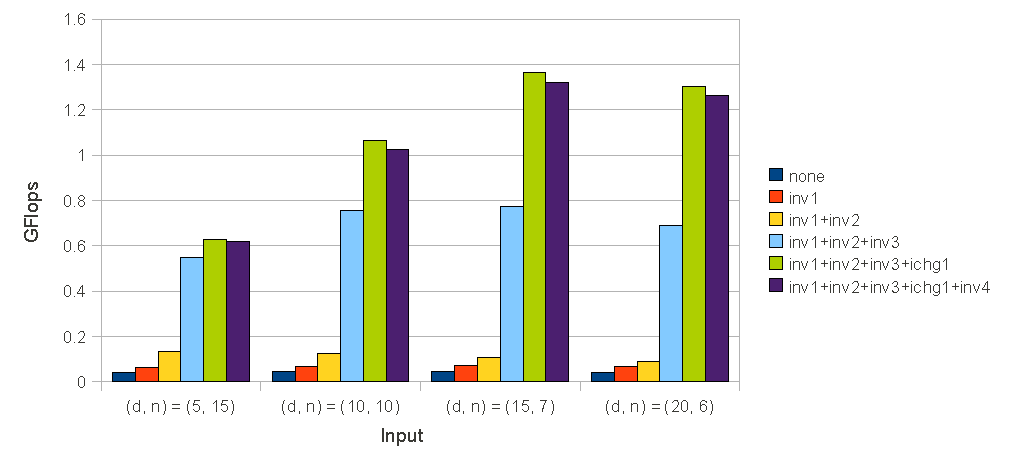
\includegraphics[width=1\linewidth]{hier_cpu} \\
    \caption{CPU}
  \end{subfigure}
  \\ \\
  \begin{subfigure}[b]{1\linewidth}
    \centering
    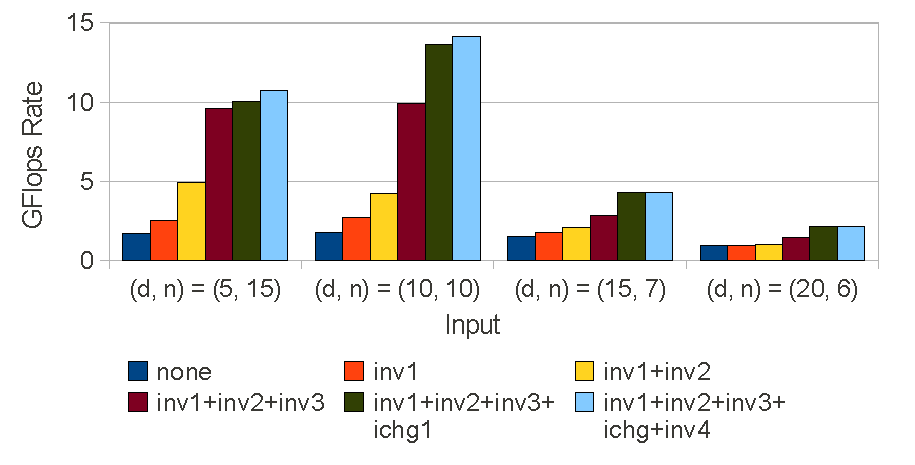
\includegraphics[width=1\linewidth]{hier_gpu}
    \caption{GPU}
  \end{subfigure}
  \caption{Impact of optimizations on the performance of \textit{hierarchization} algorithm.}
  \label{fig:hier_results}
\end{figure}

We present the impact of our optimizations for both CPU and GPU implementations
by measuring the GFlops rate and comparing with the reference baseline case
where no optimizations were applied. We start with the results obtained for the
\textit{hierarchization} algorithm, depicted in Fig.~\ref{fig:hier_results}. The
tests were done using different configurations, as displayed on the X-axis,
where $d$ is the number of dimensions and $n$ is the number of refinement
levels. We can see here that when applying all optimizations, a speedup of up to
34x is obtained for CPU and up to 8x for GPU compared to the respective baseline
cases. With the increase in the number of dimensions and the decrease of the
sparse grid size, the speedup for GPU tends to decrease. This happens because
the effects of most of the optimizations (e.g. improving caching and memory
access patterns) are visible when a high degree of parallelism is achieved,
situation which happens in the case of large grids. Thus, this context is a good
opportunity for the use of auto-tuning techniques in order to choose at runtime
the right hardware in a heterogeneous system for running the algorithm. It is
also interesting to notice that \textit{inv4} brings a drop of performance when
applied on top of the other optimizations for CPU. This means that when the
grids are smaller then it is better to actually do the computations instead of
doing memory lookups, which may result in cache misses. Lastly, we show that a
speedup of 17x is obtained for the most performant GPU version compared to the
corresponding CPU-based one and a speedup of 6.2x compared to the state of the
art GPU version \cite{Murarasu:2011:CDS:1941553.1941559}.

% \begin{figure}[h]
%   \centering
%   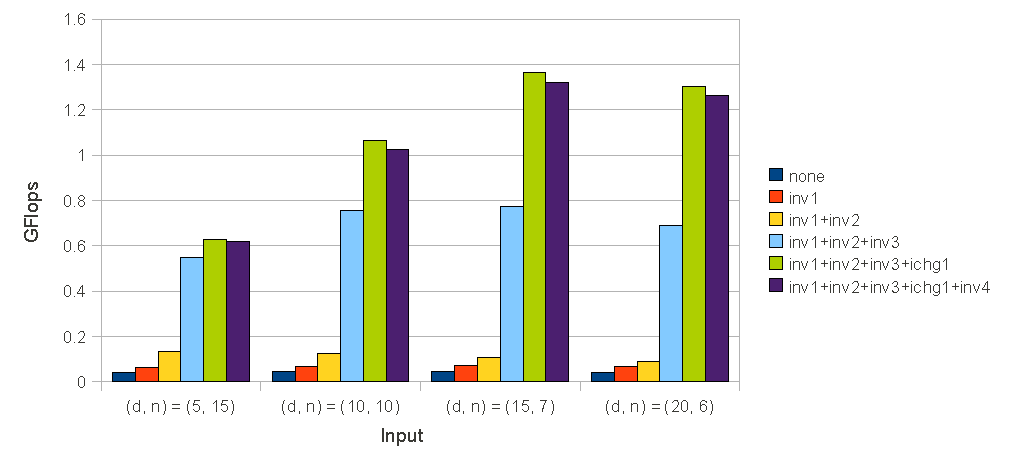
\includegraphics[width=0.5\textwidth]{hier_cpu} \\
%   \vspace{5pt}
%   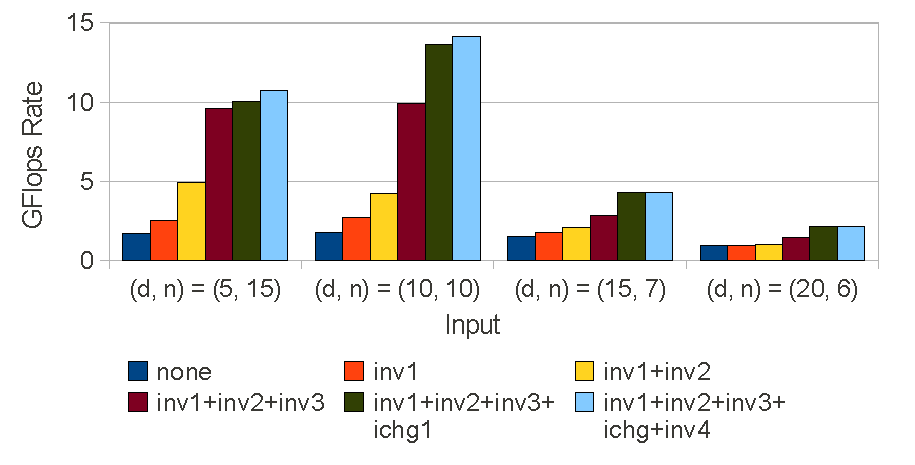
\includegraphics[width=0.5\textwidth]{hier_gpu}
%   \caption{Impact of optimizations on the performance of
%   \textit{hierarchization} algorithm for CPU (top) and GPU (bottom)}
%   \label{fig:hier_results}
% \end{figure}

For the \textit{evaluation} algorithm, we used $10^{4}$ for CPU and $10^{6}$
for GPU random points, uniformly distributed in the function domain. We
empirically observed that for CPU the GFlops rate remains constant when
increasing the number of interpolation points. The results of our tests are
presented in Fig.~\ref{fig:eval_results}. Compared to the CPU versions, the
optimizations for GPU are not that effective. The main reason for this is that
giving the high memory requirement for storing the interpolation points, we used
the GPU main memory. Although caching is performed, we believe that a higher
throughput could be obtained if we could have stored the results in shared
memory. The optimization which brings a clear speedup is \textit{sred1} showing
that division instructions are still very expensive on GPUs, fact also
emphasized by \cite{cuda}. The GPU version is 28.3x faster than the CPU
one which confirms that sparse grids interpolation technique is cache friendly
and easily parallelizable using our data structure.

\begin{figure}[t]
  \begin{subfigure}[b]{1\linewidth}
    \centering
    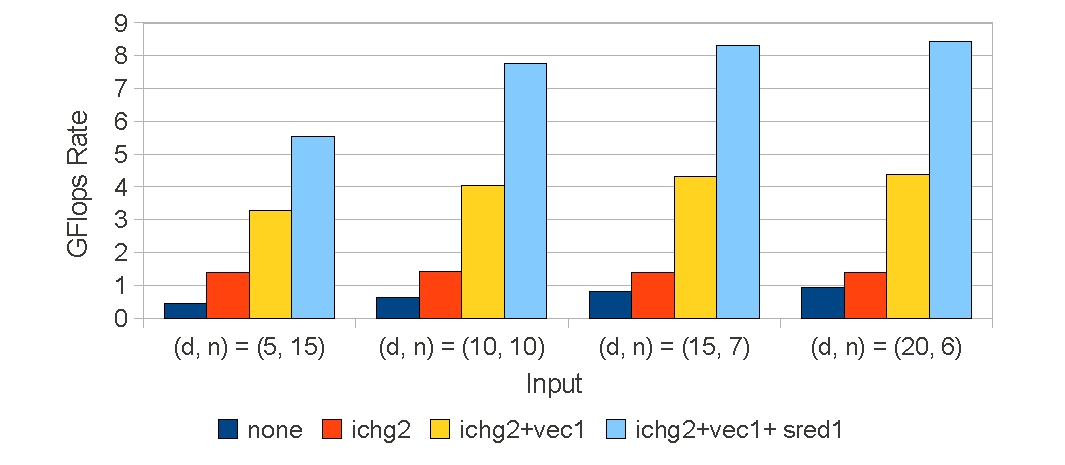
\includegraphics[width=1\linewidth]{eval_cpu} \\
    \caption{CPU}
  \end{subfigure}
  \\ \\
  \begin{subfigure}[b]{1\linewidth}
    \centering
    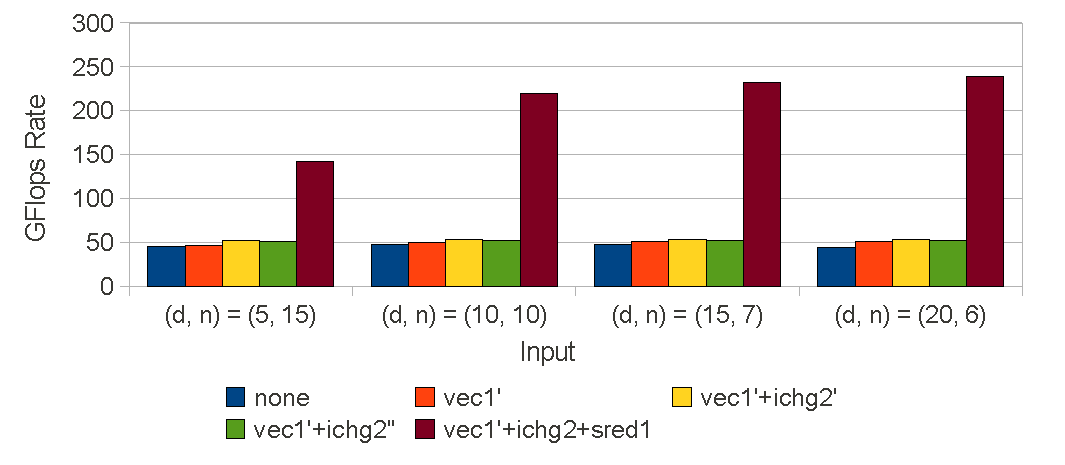
\includegraphics[width=1\linewidth]{eval_gpu}
    \caption{GPU}
  \end{subfigure}
  \caption{Impact of optimizations on the performance of \textit{evaluation} algorithm.}
  \label{fig:eval_results}
\end{figure}

% \begin{figure}[h]
%   \centering
%   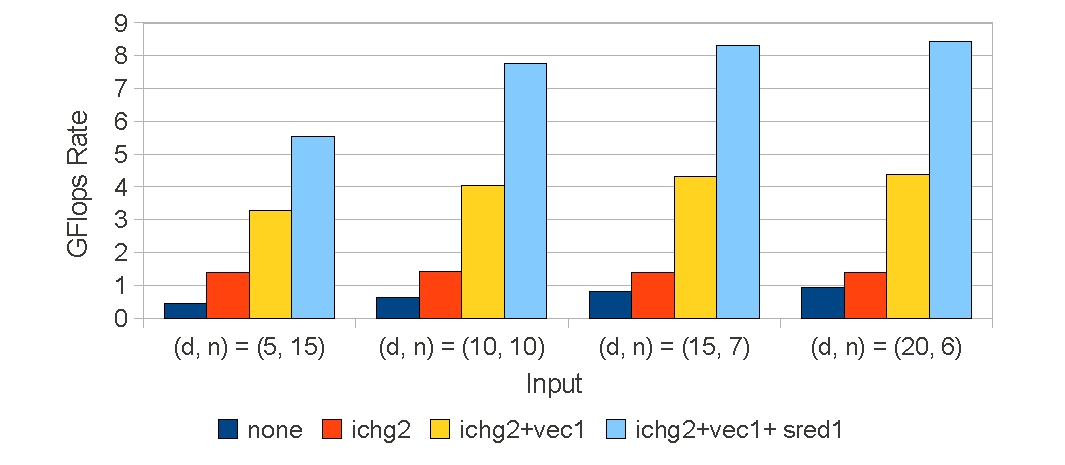
\includegraphics[width=0.5\textwidth]{eval_cpu} \\
%   \vspace{5pt}
%   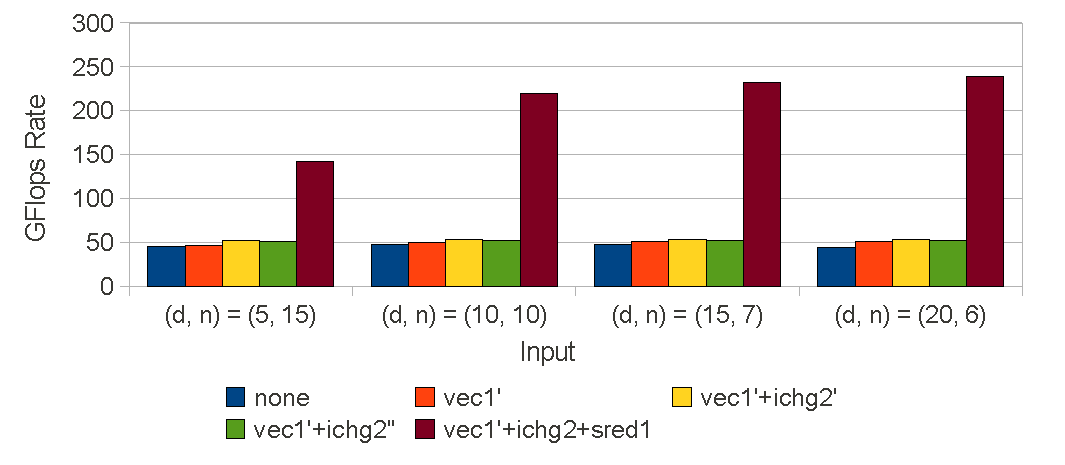
\includegraphics[width=0.5\textwidth]{eval_gpu}
%   \caption{Impact of optimizations on the performance of \textit{evaluation}
%   algorithm for CPU (top) and GPU (bottom)}
%   \label{fig:eval_results}
% \end{figure}
